% Copyright 2022  李文威 (Wen-Wei Li).
% Permission is granted to copy, distribute and/or modify this
% document under the terms of the Creative Commons
% Attribution 4.0 International (CC BY 4.0)
% http://creativecommons.org/licenses/by/4.0/

% 《代数学方法》卷一自订封面页, 由主档引入.
\begin{titlepage}
		\begin{tikzpicture}[remember picture,overlay]
			%uses the calc library
			\fill[tyellow] (current page.south west) rectangle (current page.north east);
			
			\coordinate (start) at ($(current page.east)!0.5!(current page.north east)+(1,-1)$);
			\coordinate (end)   at (current page.north west);
			\foreach \i in {0,0.01,...,1}
			{
				\coordinate (point) at ($(start)!\i!(end)$);
				\draw[tyellowlight]
				($(point)+(310*\i:6)$)--
				($(point)+(310*\i+120:6)$)--
				($(point)+(310*\i+240:6)$)--
				($(point)+(310*\i:6)$);
			}
			\coordinate (start) at (current page.south west);
			\coordinate (end)   at (current page.east);
			\foreach \i in {0,0.02,...,1}
			{
				\coordinate (point) at ($(start)!\i!(end)$);
				\draw[tyellowlight]
				($(point)+(310*\i:10)$)--
				($(point)+(310*\i+120:10)$)--
				($(point)+(310*\i+240:10)$)--
				($(point)+(310*\i:10)$);
			}%背景绘制,需要用到setting里面的tikzlibrary中的部分.
			\node (title)
			[shape=rectangle, 
			fill=tbluedark,
			outer sep=2em,
			inner sep=2em,
			minimum height=12em, 
			minimum width=\paperwidth, 
			align=flush right, 
			text=white,
			text width=0.8\paperwidth,
			anchor=north
			] 
			at ($(current page.center)!0.6!(current page.north)$)
			{
				\fontsize{5em}{4em}
				\fontfamily{lmss}
				\selectfont
				Metaphysics\par
			};%书名位置
			
			\node (author)
			[
			fill=tblue,
			inner sep=0.75em,
			align=flush right,
			text=white,
			anchor=east
			]
			at ($(title.north east)-(0.125\paperwidth,0)$)
			{
				\fontsize{3em}{2.5em}
				\fontfamily{lmss}
				\selectfont
				Bufan Zheng\par
			};
			\node
			[
			fill=tblue,
			inner sep=0.75em,
			align=flush left,
			text=tblue,
			anchor=west,
			xshift=-2mm
			]
			at (author.east)
			{
				\fontsize{3em}{2.5em}
				\fontfamily{lmss}
				\selectfont
				\phantom{Bufan Zheng}\par
			};%作者名字位置
			
			\node (subtitle)
			[
			text=black,
			align=flush right,
			anchor=north east         
			]
			at ($(title.south east)+(-0.14\paperwidth,0.5)$)
			{
				\fontsize{1.5em}{1em}
				\fontfamily{lmss}
				\selectfont
				I don't know which Edition\par
			};%第几版的位置
			
			\node (coverinfo)
			[text=black]
			at ($(current page.center)!0.825!(current page.south)$)
			{
				\fontsize{1.5em}{1em}
				\fontfamily{lmss}
				\selectfont
				Revised and modernized edition by \par
			};%logo的位置
			\node
			[text=black]
			at ($(current page.center)!0.9!(current page.south)$)
			{
				\raisebox{1.1em}{
					\fontsize{1.5em}{1em}\selectfont\LaTeX{}\par
				}
			};%我改的名字的位置
			\node (coverpic)
			at ($(title.south)!0.5!(coverinfo.north)$)
			{
				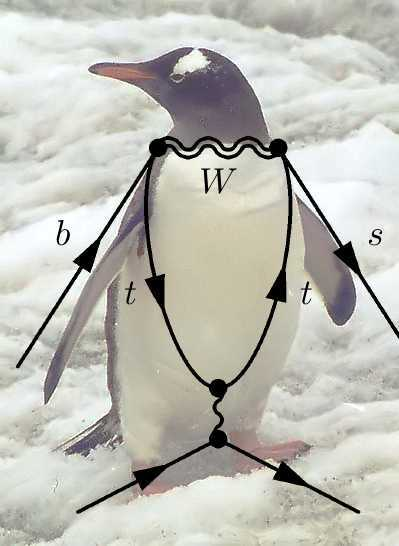
\includegraphics[width=0.3\linewidth]{figs/penguin.jpeg}
			};
			
			
		\end{tikzpicture}

\clearpage	% 进入内页
\begin{center}
	\Large{\sffamily\bfseries\thmheiti 网络版 \\ 从未修订,将来也不会} \\ \vspace{2em}
	\Large{\sffamily\bfseries\thmheiti 编译日期: \today} \\ \vspace{1em}
%	版面: B5 (176×250mm) \\ \vspace{1em}
	本书已由Dinner教育出版社发行 \\
	(2004 年 4 月第 10 版) \\
	\texttt{ISBN: 4210xxxxxxxxxxxxxx}
\end{center}
\begin{figure}[H]
	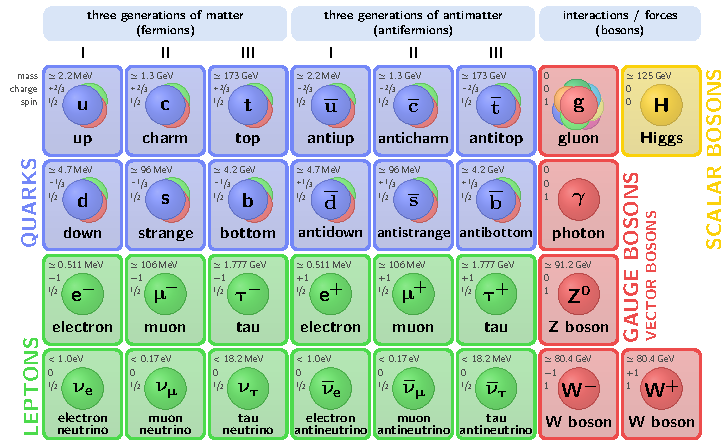
\includegraphics[width=\linewidth]{figs/sm.pdf}
\end{figure}
\vfill

\begin{flushleft} \small
	郑卜凡 \\
	个人Github主页: \href{https://github.com/WHUZBF}{WHUZBF} \\
\end{flushleft}
\vspace{1.5em}
\begin{tabular*}{\textwidth}{ccc}
	
\includegraphics{ccby.png}
	& \begin{minipage}[b]{0.6\textwidth}
		\small\sffamily
		本作品采用知识共享 署名 4.0 国际 许可协议进行许可. 访问 \url{http://creativecommons.org/licenses/by/4.0/} 查看该许可协议.
	\end{minipage}
\end{tabular*}

\cleardoublepage
\end{titlepage}
